\section{Measurement errors estimation}
\label{sec:errors}

Notation used in this section is based on the \emph{BIPM} document on uncertainty in
measurements\cite{bipm_errors}\vspace{0.1cm}:

\begin{tabular}{p{1cm} p{14cm}}
 $q_k$ & single sample of the measured quantity \emph{q}\\
 $\bar{q}$ & arithmetic mean calculated from N independent observations of quantity \emph{q}:\newline $\bar{q} = \frac{1}{N}\sum\limits_{k=1}^N q_k$\\
 $s^2 (q_k)$ & experimental variance of the \emph{q} observation calculated using N samples:\newline $s^2(q_k) = \frac{1}{N-1}\sum\limits_{j=1}^N (q_j - \bar{q})^2$\\
 
 $s^2 (\bar{q})$ & experimental variance of the mean value of \emph{q}:
 $s^2 (\bar{q}) = \frac{s^2(q_k)}{N}$\\
 
 $s(\bar{q})$ & experimental standard deviation of the mean\\
 $u^2(q)$ & uncertainty of the quantity \emph{q} estimation: $u^2(q) = s^2(\bar{q})$\\
 $u_c^2(y)$ & combined standard uncertainty of the value \emph{y} determined from N other quantities $y = f(x_1, x_2, ..., x_N)$:
 	$u_c^2(y) = \sum\limits_{n=1}^N \left( \frac{\partial f}{\partial x_n}\right) ^2 u^2(x_i)$ \\
\end{tabular}

\subsection{Fiber latency measurement}
\label{subsec:errors:filat}

In section \ref{subsec:refiber} the latency of the fiber is calculated based
on the round trip delays after subtracting the bitslides $\epsilon_M$,
$\epsilon_S$ ($delay'_{MM}$):
\begin{align}
	\delta_1 = delay'_{MM3} - delay'_{MM2}\\
	\delta_2 = delay'_{MM3} - delay'_{MM1}
\end{align}
WR Devices currently used know the precise value of a bitslide, which comes
directly from the GTP/GTX SerDes. The inaccuracy of the bitslide can be ignored,
and the uncertainty of $delay_{MM}$ treated as the uncertainty of
$delay'_{MM}$.\\

{\bf Note:} If an alternative implementation needs to perform an on-line
calibration to measure the delays of an external Ethernet PHY, the uncertainty
of such measurement would have to be added to the considerations below.\\

The combined standard uncertainty of the fiber latency measurement can be estimated
with the formula:
\begin{align}
	\label{equ:errors:filat}
	u_c^2(\delta_1) &= \left( \frac{\partial \delta_1}{\partial delay_{MM3}} \right)^2 u^2(delay_{MM3}) + \left( \frac{\partial \delta_1}{\partial delay_{MM2}} \right)^2 u^2(delay_{MM2}) \nonumber \\
	&= u^2(delay_{MM3}) + u^2(delay_{MM2})
\end{align}

\noindent That means, we have to know the uncertainty of the round-trip delay
($delay_{MM}$) calculated by the WR PTP software.
\renewcommand{\arraystretch}{1.2}
\begin{table}[ht]
	\begin{center}
  \resizebox{\textwidth}{!}{
	\begin{tabular}{|p{2cm}|r|r|r|r|r|r|}
	\hline
	\emph{device} & \emph{fiber len.} & $\overline{del_{MM}}$ [ps] & $s^2(del_{MM})$ [ps$^2$] & $s^2(\overline{del_{MM}})$ [ps$^2$] & $s(del_{MM})$ [ps] & $s(\overline{del_{MM}})$ [ps]\\
	\hline \hline
	\multirow{3}{*}{WR Switch} & 5 m & 962151 & 5.38 & 0.054 & 2.32 & 0.23\\
	\cline{2-7}
	& 5 km & 51333653 & 8.53 & 0.085 & 2.92 & 0.29\\
	\cline{2-7}
	& 5+ km & 51377317 & 8.97 & 0.090 & 2.99 & 0.30 \\
	\hline
	WRPC / & 5 m & 712223 & 17.58 & 0.176 & 4.19 & 0.42\\
	\cline{2-7}
	SPEC & 5 km & 51085804 & 21.31 & 0.21 & 4.61 & 0.46 \\
	\cline{2-7}
	& 5+ km & 51138454 & 23.02 & 0.23 & 4.80 & 0.48 \\
	\hline
	\end{tabular}
  }
	\caption{Experimental uncertainties of $delay_{MM}$ for various WR Devices based on N=100 observations made in 1s intervals}
	\label{tab:errors:dmm}
	\end{center}
\end{table}
\renewcommand{\arraystretch}{1}
Table \ref{tab:errors:dmm} presents the experimental $delay_{MM}$ uncertainties
measured for two WR Switches and two SPEC cards running the White Rabbit PTP
Core. The measurement was performed with a short (5 m) fiber, long (5 km)
fiber and both fibers connected together (5+ km). Table shows that the standard
deviation is at the picosecond level even when a single sample of $delay_{MM}$
estimation is taken instead of the mean value.\\

Based on those values and using equation \ref{equ:errors:filat} we can calculate
the uncertainty of a fiber latency estimation made with two WR Switches and
using a single sample or an averaged $delay_{MM}$:
\begin{align}
	\label{equ:errors:f1lat}
  u_c^2(\delta_1) &= s^2(del_{MM5+km}) + s^2(del_{MM5km}) = 17.5 [ps^2]\\
	u_c^2(\delta_2) &= s^2(del_{MM5+km}) + s^2(del_{MM5m}) = 14.4 [ps^2]\\
	u_c^2(\bar{\delta_1}) &= s^2(\overline{del_{MM5+km}}) + s^2(\overline{del_{MM5km}}) = 0.175 [ps^2]\\
	u_c^2(\bar{\delta_2}) &= s^2(\overline{del_{MM5+km}}) + s^2(\overline{del_{MM5m}}) = 0.144 [ps^2]
\end{align}

These uncertainties are negligible for the current WR needs. However, the
latency of the fiber also changes with the temperature, which may be the source
of additional measurement error. Figure \ref{fig:errors:deltemp} shows how the
round-trip delay changes over time for the two fiber cables: 5km and 5m. 

\begin{center}
\begin{figure}[ht]
a)
\begin{minipage}{.5\textwidth}
	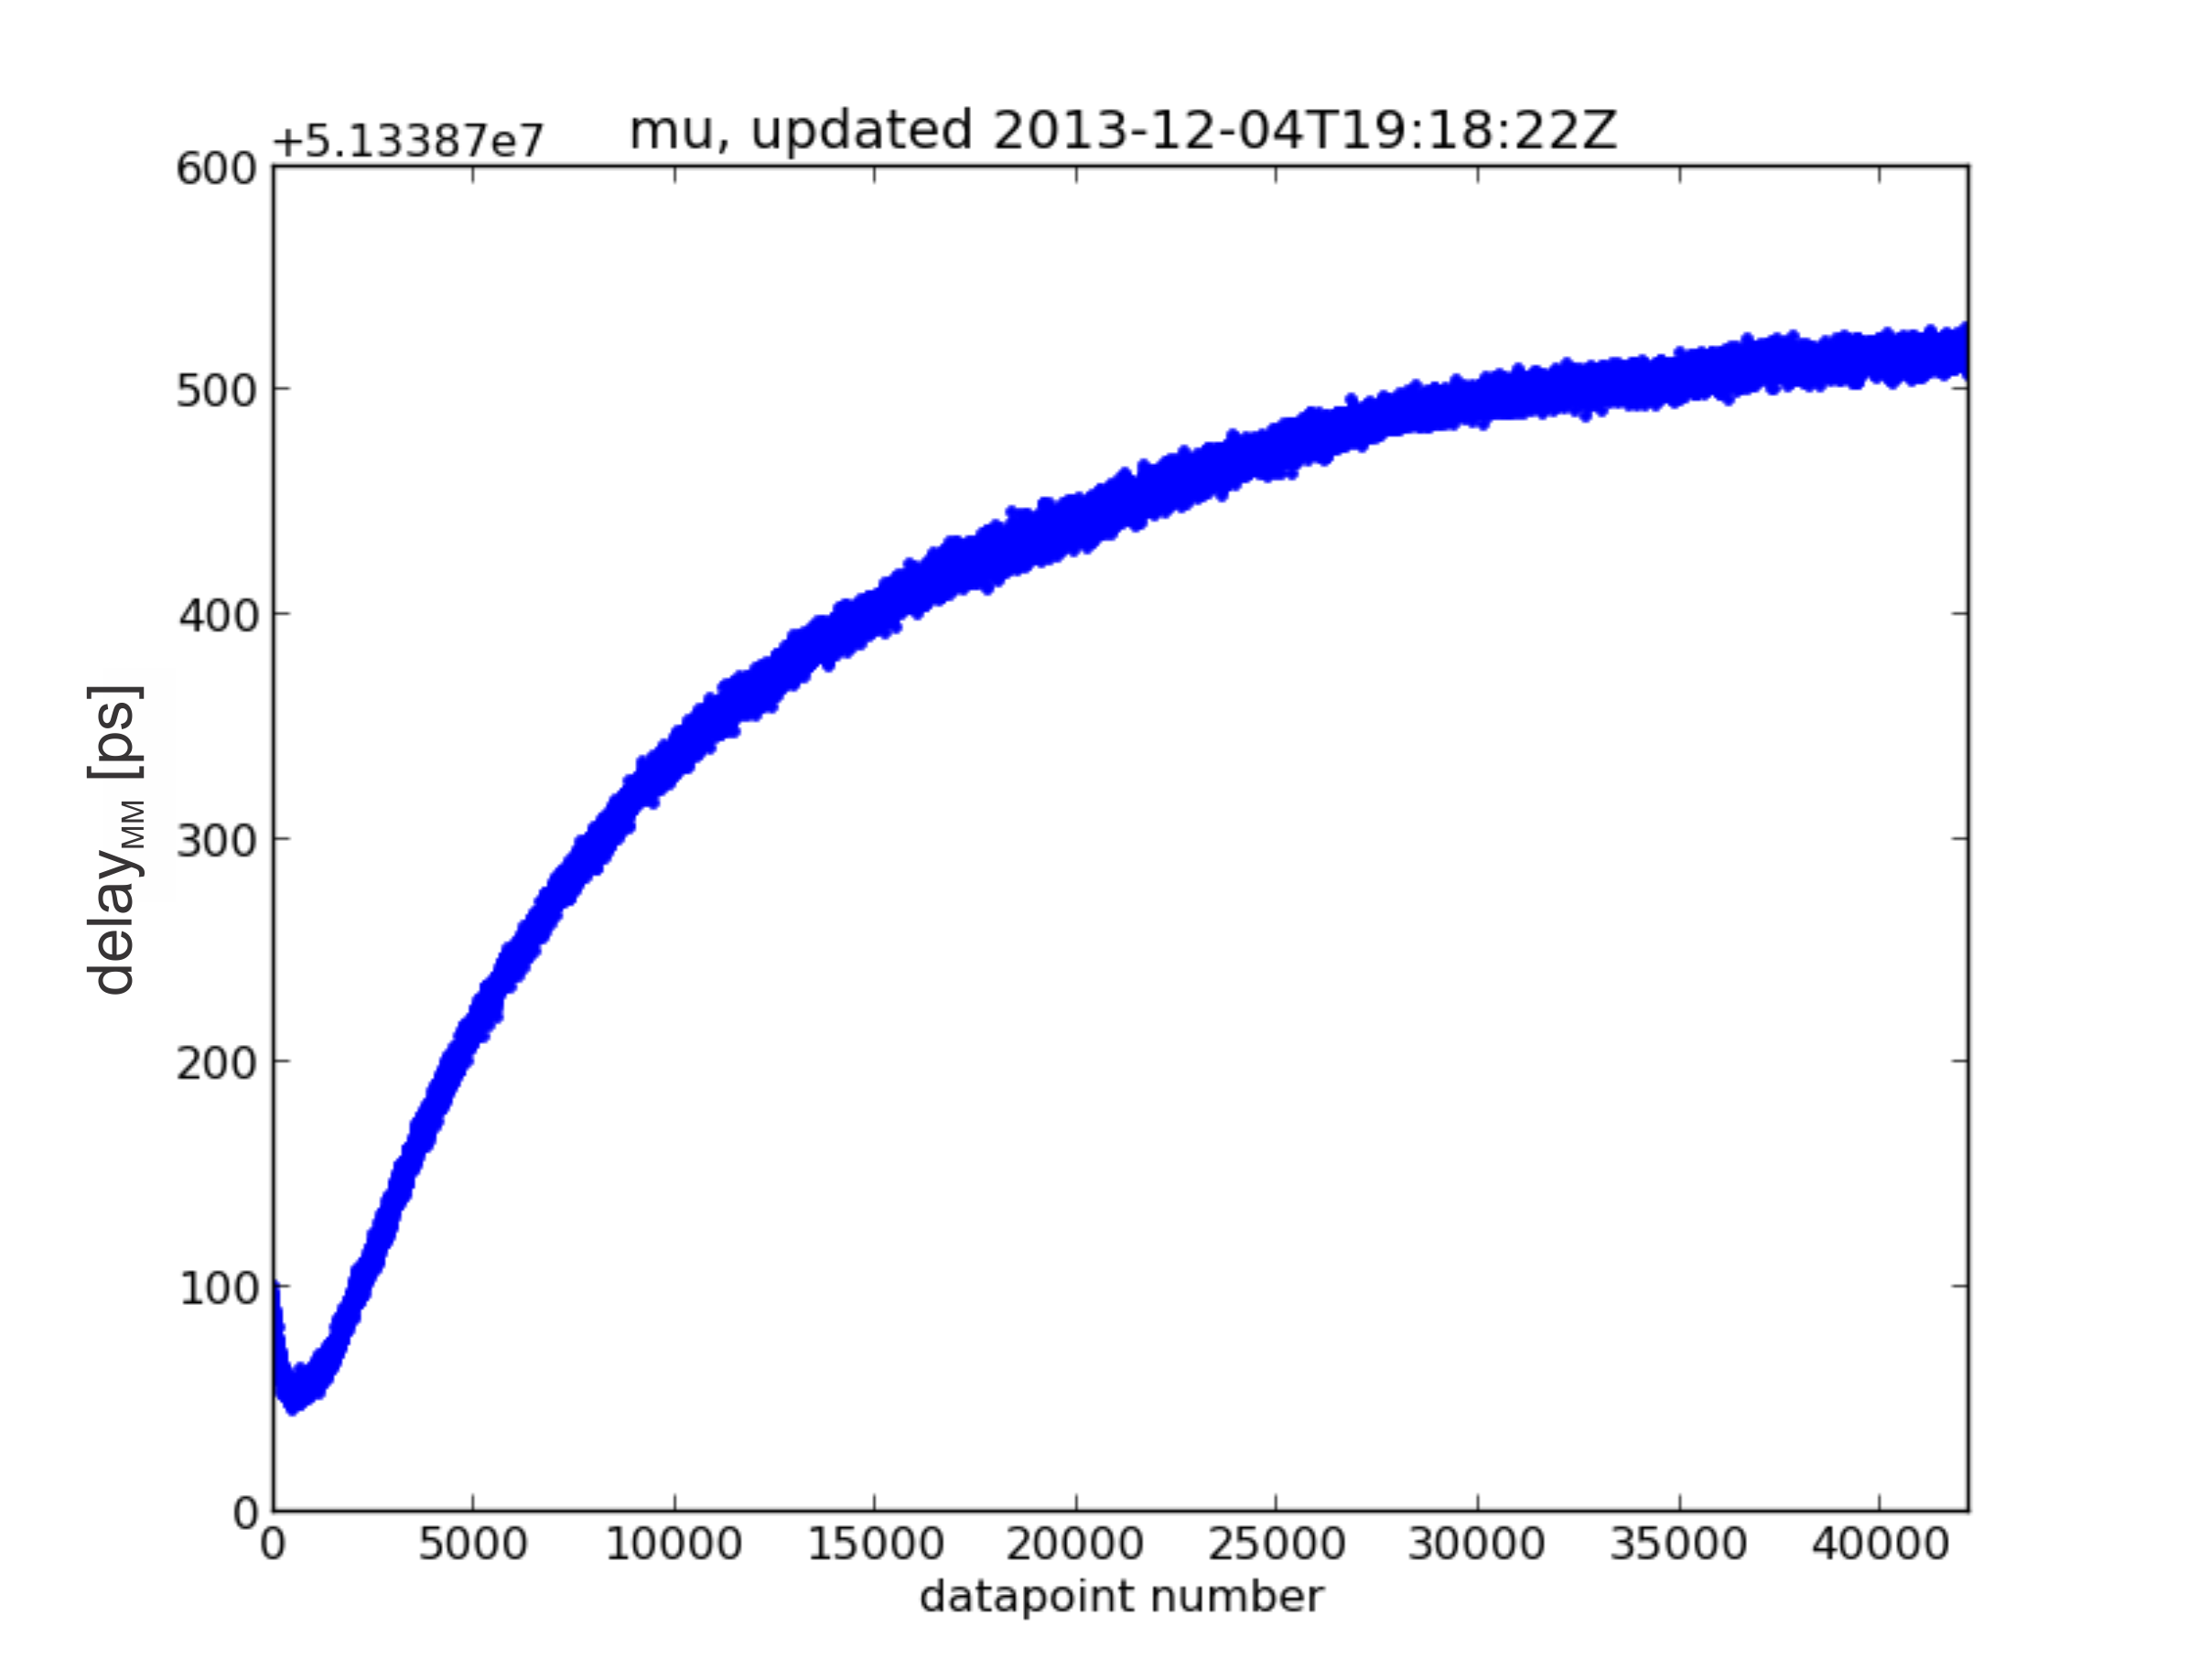
\includegraphics[width=\textwidth]{calibration/rtt_long.png}
\end{minipage}
b)
\begin{minipage}{.5\textwidth}
	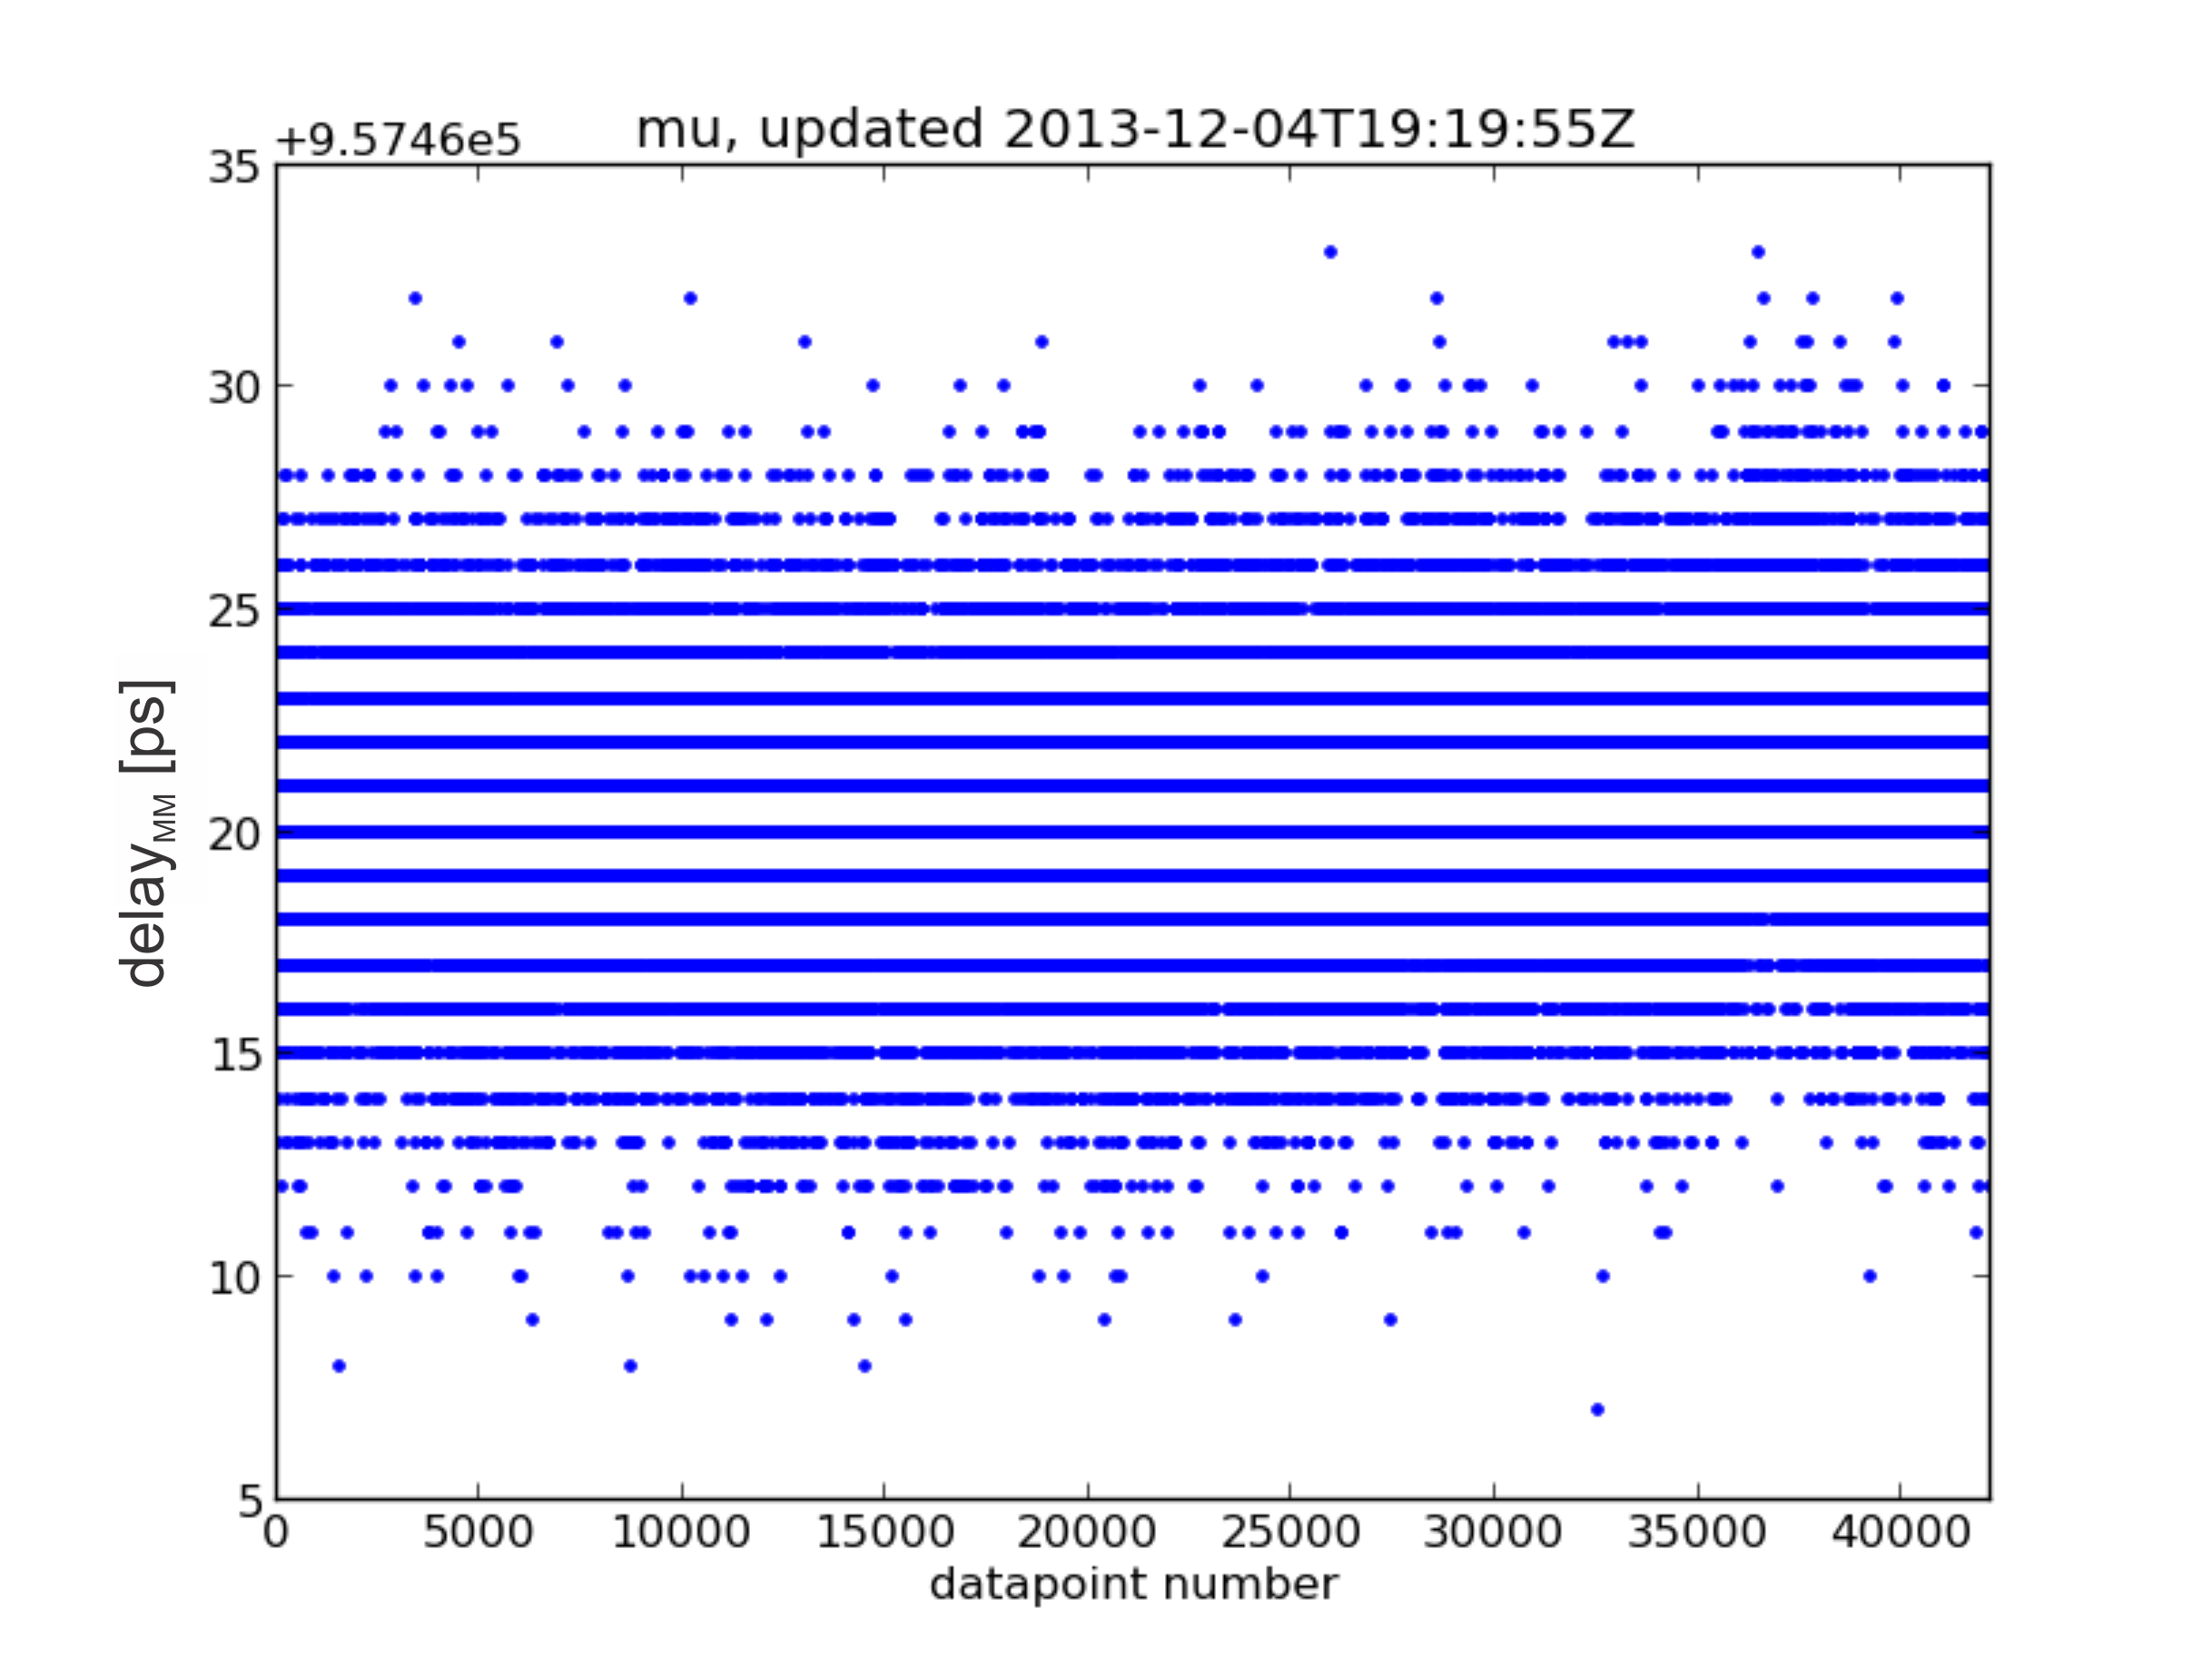
\includegraphics[width=\textwidth]{calibration/rtt_short.png}
\end{minipage}
\caption{$delay_{MM}$ of 5 km (a) and 5 m (b) fiber logged for almost 12 hours using two WR Switches}
\label{fig:errors:deltemp}
\end{figure}
\end{center}

It is noticeable, that the latency of the long fiber (5 km) varies much more
over time (caused by the temperature change) than the latency of the short one.
Table \ref{tab:errors:deltemp} presents the variances calculated for this almost
12-hour data set.
\renewcommand{\arraystretch}{1.2}
\begin{table}[ht]
	\begin{center}
	\begin{tabular}{|r|r|r|}
	\hline
  \emph{fiber len.} & $s^2(\delta)$ [ps$^2$] & $s(\delta)$ [ps]\\
	\hline
	5 m & 7.92 & 2.81\\
	\hline
	5 km & 16273 & 128\\
	\hline
	\end{tabular}
	\caption{Long term uncertainty of $delay_{MM}$ measurement caused by temperature fluctuations}
	\label{tab:errors:deltemp}
	\end{center}
\end{table}
\renewcommand{\arraystretch}{1}

This means, the latency of the long fiber measured once, may not be valid
anymore when used for the calibration procedures few days later - in a different
ambient temperature. There are two conclusions from this fact:
\begin{itemize}
  \item when you want to measure the $\alpha$ parameter of a long fiber, perform
    the latency measurement (section \ref{subsec:refiber}) prior the
    oscilloscope measurements (section \ref{subsec:fiasym});
  \item use a short (few meters) fiber to calibrate a WR Calibrator and all WR
    Devices (sections \ref{sec:procedure:calibrator}, \ref{subsec:devices}),
    then the latency measurement of the short fiber performed only once will be
    accurate enough independently of the ambient temperature.
\end{itemize}


%%%%%%%%%%%%%%%%%%%%%%%%%%%%%%%%%%%%%%%%%%%%%%%%%%%%%%%%%
\subsection{Fiber asymmetry}
\label{subsec:errors:fiasym}

As described in section \ref{subsec:fiasym}, the asymmetry of the fiber is
expressed with the $\alpha$ parameter:
\begin{equation}
	\alpha = \frac{2(skew_{PPS2}-skew_{PPS1})}{\frac{1}{2}\delta - (skew_{PPS2}-skew_{PPS1})}
\end{equation}

\noindent The uncertainty of $\alpha$ depends on:
\begin{itemize}
	\item the uncertainty of the fiber latency estimation ($u^2(\delta)$)
  \item the uncertainty of the 1-PPS skew between the two WR Devices ($u^2(skew_{PPS})$).
\end{itemize}
The former was already addressed in the previous section
(\ref{subsec:errors:filat}). The uncertainty of the 1-PPS skew between two WR
Devices is the measuring instrument uncertainty subtracted from the uncertainty
of 1-PPS skew measurement done with this instrument:
\begin{equation}
  \label{equ:fiasym:skewPPS}
  u^2(skew_{PPS}) = u^2(meas_{PPS}) - u^2(instr.)
\end{equation}

The uncertainty of the instrument (e.g. oscilloscope) can be taken from
its datasheet or measured in the lab. The measurement can be done by feeding
the same signal to both oscilloscope channels (fig.\ref{fig:errors:osc_jitter}).
You can use either a 50 $\Omega$ splitter (fig.\ref{fig:errors:osc_jitter}.1) or
make a daisy-chain connection (fig.\ref{fig:errors:osc_jitter}.2). The
latter requires setting one oscilloscope channel to high impedance and the
other to 50 $\Omega$ termination. The signal fed to an oscilloscope can be taken
from a signal generator (e.g. Agilent 33250A) or it can be also a 62.5MHz clock
output taken from a WR Switch.
\begin{figure}[ht]
	\begin{center}
	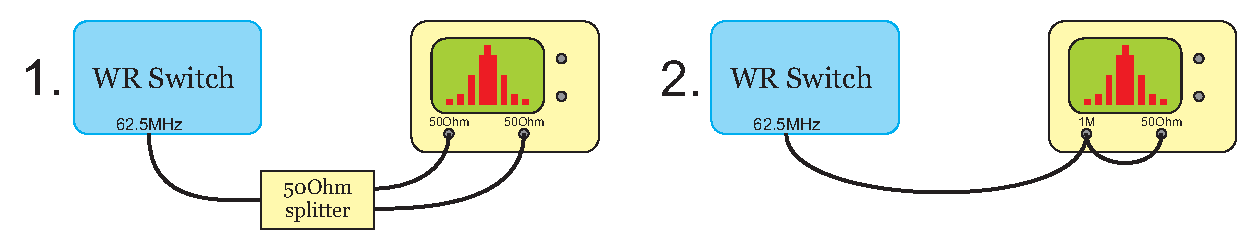
\includegraphics[width=\textwidth]{calibration/oscil_meas.pdf}
	\caption{Measuring internal jitter of an oscilloscope}
	\label{fig:errors:osc_jitter}
	\end{center}
\end{figure}
An example measurement done this way for the \emph{Lecroy Wavepro 7300A}
oscilloscope using a 62.5MHz clock output from a free-running WR Switch is
presented in figure \ref{fig:errors:lecroy_jitter}.
\begin{figure}
	\begin{center}
	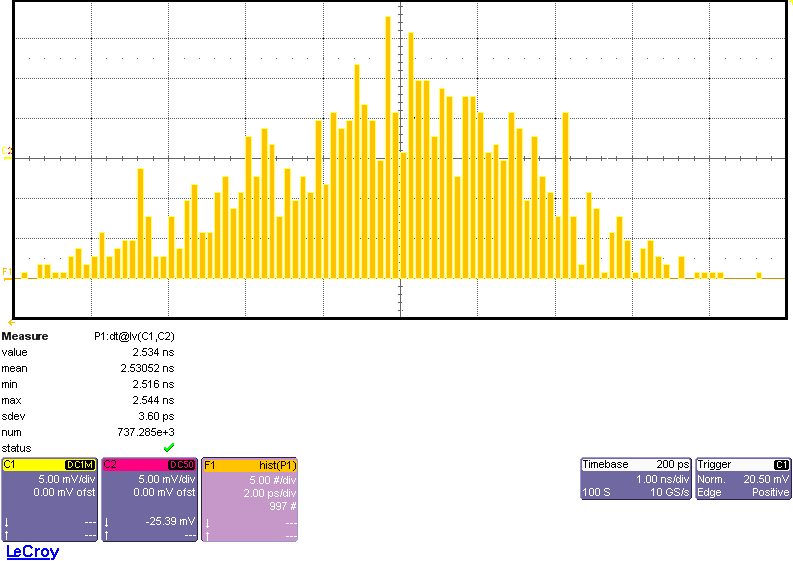
\includegraphics[width=.8\textwidth]{calibration/lecroy_7300_jitter.png}
	\caption{Uncertainty of LeCroy Wavepro 7300A oscilloscope}
	\label{fig:errors:lecroy_jitter}
	\end{center}
\end{figure}
For our considerations the uncertainty of the measuring instrument is:
\begin{align}
	u(instr.) &= 3.6 [ps]\\
	\label{equ:errors:ulecroy}
  u^2(instr.) &= 12.96 [ps^2]
\end{align}

\noindent For comparison, the uncertainty of a \emph{Rhode\&Schwarz RTO1004}
oscilloscope measured the same way is $u^2(instr.) = 30.80 [ps^2]$\\

The next step is to determine the total uncertainty of the 1-PPS skew measurement
($u^2(meas_{PPS})$). It can be done with an oscilloscope by logging the 1-PPS
skew between two synchronized WR Devices. The standard deviation and the
variance can be calculated based on these samples. Parameters measured with the
\emph{Lecroy Wavepro 7300A} for two WR Switches v3.3, two SPECs running the WR
PTP Core v2.1 and the WR Switch with SPEC are presented in table
\ref{tab:errors:ppsjitter}.
\begin{table}[ht]
	\begin{center}
	\begin{tabular}{|l|c|c|}
		\hline
    \emph{devices} & $u(meas_{PPS}) [ps]$ & $u^2(meas_{PPS}) [ps^2]$\\
		\hline
		WR Switch - WR Switch & 9.33 & 87.05\\
		WR Switch - SPEC & 19.37 & 375.20\\
	  SPEC - SPEC & 26.79 & 717.70\\
		\hline
	\end{tabular}
	\end{center}
  \caption{Total jitter of 1-PPS skew measurement}
	\label{tab:errors:ppsjitter}
\end{table}

Using equation \ref{equ:fiasym:skewPPS}, values from \ref{equ:errors:ulecroy}
and table \ref{tab:errors:ppsjitter} the uncertainty of the 1-PPS skew between
two WR Devices can be calculated. The uncertainties for various configurations
are collected in table \ref{tab:errors:skewpps}.
\begin{table}[ht]
  \begin{center}
    \begin{tabular}{|l|c|c|}
      \hline
      \emph{devices} & $u(skew_{PPS}) [ps]$ & $u^2(skew_{PPS}) [ps^2]$\\
      \hline
      WR Switch - WR Switch & 8.61  & 74.09\\
           WR Switch - SPEC & 19.03 & 362.24\\
                SPEC - SPEC & 26.55 & 704.74\\
      \hline
    \end{tabular}
  \end{center}
  \caption{Jitter of 1-PPS skew produced by various WR devices}
  \label{tab:errors:skewpps}
\end{table}

These uncertainties can be used then to calculate the uncertainty of the
$\alpha$ parameter estimated according to step \ref{subsec:fiasym} of the
calibration procedure. To simplify the equations, we introduce a new parameter
$s$ with uncertainty $u^2(s)$:
\begin{align}
	s &= skew_{PPS2} - skew_{PPS1}\\
  u^2(s) &= u^2(skew_{PPS2}) + u^2(skew_{PPS1}) = 2 \cdot u^2(skew_{PPS})
\end{align}

{\bf Note:} If two exactly the same WR Devices (with the same firmware version)
are used for this step of the calibration, then the measured $skew_{PPS1}$ will
be equal to 0 ps. That is because there won't be any asymmetry of the hardware
for a given connection and the asymmetry of a few meters long fiber is
negligible. In such case doing only one measurement of the 1-PPS skew
($skew_{PPS2}$) is enough and estimations $s$, $u^2(s)$ can be simplified:
\begin{align}
	s &= skew_{PPS2}\\
  u^2(s) &= u^2(skew_{PPS})
\end{align}

\noindent By putting parameter $s$ to the $\alpha$ equation we get a new
formula for estimating the uncertainty:
\begin{equation}
	\alpha = \frac{2\cdot s}{\frac{1}{2}\delta - s}
\end{equation}

\noindent The combined standard uncertainty of the $\alpha$ is then estimated as:
\begin{align}
	\label{equ:errors:ualpha}
	u_c^2(\alpha) &= \left( \frac{\partial \alpha}{\partial s} \right)^2 u^2(s) + \left(
	\frac{\partial \alpha}{\partial \delta} \right)^2 u^2(\delta) \nonumber\\
  & = \left( \frac{\delta}{(\frac{1}{2}\delta - s)^2} \right)^2 u^2(skew_{PPS}) + \left(
	\frac{-s}{(\frac{1}{2}\delta - s)^2} \right)^2 u^2(\delta)
\end{align}

Taking a look at the $\left( \frac{\partial \alpha}{\partial s} \right)$ factor,
we can conclude that the influence of the 1-PPS skew uncertainty is smaller when
the latency is greater (fiber is longer):
\begin{equation}
	\lim_{\delta \to \infty} \left( \frac{\partial \alpha}{\partial s} \right) = 0
\end{equation}

As an example we can calculate the combined uncertainty of $\alpha$ using
equation \ref{equ:errors:ualpha} for a 5 km fiber measured with the \emph{LeCroy
Wavepro 7300A} and two WR Switches:
\begin{align}
  &\delta = 50421913 [ps] \hspace{1cm} s = 3243 [ps]\nonumber \\
  &u^2(\delta) = 14.4 [ps^2] \hspace{1cm} u^2(skew_{PPS}) = 74.09 [ps^2] \nonumber \\
	\label{equ:errors:alpha}
	\alpha &= 2.573e-4 \\
	\label{equ:errors:unc_alpha}
  u_c^2(\alpha) &= 4.665e-13\\
	\label{equ:errors:stdev_alpha}
  u_c(\alpha) &= 0.0068e-4
\end{align}

The uncertainty of $\alpha$ may cause about \emph{9 ps} of uncompensated
asymmetry in a 5km link. It can be calculated by subtracting the WR PTP
$delay_{MS}$ estimations for the measured $\alpha$ (equation
\ref{equ:errors:alpha}) and for $\alpha$ distorted by its standard deviation:
\begin{equation}
	error = delay_{MS}(\alpha \pm u_c(\alpha)) - delay_{MS}(\alpha) \approx 9 [ps]
\end{equation}

%%%%%%%%%%%%%%%%%%%%%%%%%%%%%%%%%%%%%%%%%%%%%%%%%%%%%%%%%
\subsection{Calibrator pre-calibration}
The parameters of a WR Calibrator determined in the calibration procedure depend
on two experimental values:
\begin{itemize}
	\item round trip delay $delay_{MM}$
	\item fiber latency $\delta$
\end{itemize}

The combined standard uncertainties of a transmission and reception delay are the
same and can be estimated in a similar way as in previous sections:
\begin{align}
	u_c^2(\Delta_{TX}) &= u_c^2(\Delta_{RX}) \\
	u_c^2(\Delta_{TX}) &= \left( \frac{\partial \Delta_{TX}}{\partial delay_{MM}}
	\right)^2 u^2(delay_{MM}) + \left( \frac{\partial \Delta_{TX}}{\partial
	\delta} \right)^2 u^2(\delta) \nonumber\\
	&= \frac{1}{16} u^2(delay_{MM}) + \frac{1}{16} u^2(\delta)
\end{align}

As an example we can calculate the combined uncertainty of $\Delta_{TX}$ when
port \emph{1} of the WR Switch is selected to be a WR Calibrator and the calibration is
done with the 5m fiber used in the previous steps. To evaluate the worst case, the
uncertainties for single sample measurements (not means) are used here
($s^2(del_{MM})$ from table \ref{tab:errors:dmm} and $u^2_c(\delta_1)$ from
equation \ref{equ:errors:f1lat}):
\begin{align}
	u_c^2(\Delta_{TX}) &= \frac{1}{16} \cdot 5.38 + \frac{1}{16} \cdot 17.5  =
  1.43 [ps^2]\\
	u_c(\Delta_{TX}) &= 1.20 [ps]
\end{align}

%%%%%%%%%%%%%%%%%%%%%%%%%%%%%%%%%%%%%%%%%%%%%%%%%%%%%%%%%
\subsection{WR Device calibration}
The last step of the calibration procedure depends on all the previous stages.
First, we should estimate the uncertainty of the coarse (average) transmission
and reception delays of a WR Device. Rewriting equation
\ref{equ:devices:coarsedtxrx} and omitting the bitslide value gives us equation
\ref{equ:errors:devices:dtxrx} which is used for the uncertainty
estimation (\ref{equ:errors:devices:udtxrx}). The fixed delays of the WR
Calibrator are represented by symbols $\Delta_{TXC}$ and $\Delta_{RXC}$.
\begin{align}
	\label{equ:errors:devices:dtxrx}
	\Delta'_{TXS} &= \Delta'_{RXS} = \frac{1}{2}(delay_{MM} - \Delta_{TXC} -
	\Delta_{RXC} - \delta)\\
	\label{equ:errors:devices:udtxrx}
	u^2(\Delta'_{TXS}) &= \left( \frac{\partial \Delta'_{TXS}}{\partial delay_{MM}} \right)^2 u^2(delay_{MM}) +
	2 \cdot \left( \frac{\partial \Delta'_{TXS}}{\partial \Delta_{TXC}} \right)^2 u^2(\Delta_{TXC}) +
	\left( \frac{\partial \Delta'_{TXS}}{\partial \delta} \right)^2 u^2(\delta) \nonumber\\
	&= \frac{1}{4} u^2(delay_{MM}) + \frac{1}{2} u^2(\Delta_{TXC}) + \frac{1}{4} u^2(\delta)
\end{align}

For the case when the WR Switch is the calibrator, the WRPC running on a SPEC is
the WR Device under calibration and the connection is made with a short fiber,
the uncertainty of the coarse fixed delay is:
\begin{align}
	u^2(\Delta'_{TXS}) &= u^2(\Delta'_{RXS}) = \frac{1}{4} \cdot 17.58 +
  \frac{1}{2} \cdot 1.43 + \frac{1}{4} \cdot 17.5 = 9.49 [ps^2]\\
	u(\Delta'_{TXS}) &= u(\Delta'_{RXS}) = 3.08 [ps]
\end{align}\\

The second part of the WR Device calibration uses the 1-PPS skew readout from
the oscilloscope as the correction value $\beta$ to compensate fixed delay
asymmetry. The uncertainty of the estimation of $\beta$ is then the sum of two
factors: the uncertainty of the 1-PPS skew measurement (the same as in
\ref{subsec:errors:fiasym}) and the uncertainty of the one way delay
($delay_{MS}$) estimation in the WR PTP software:
\begin{equation}
	\label{equ:errors:ubeta}
	u^2(\beta) = u^2(skew_{PPS}) + u^2(delay_{MS})
\end{equation}

\noindent Knowing the formula used by the WR PTP software for estimating $delay_{MS}$:
\begin{equation}
	delay_{MS} = \frac{1+\alpha}{2+\alpha}(delay_{MM} - \Delta) + \Delta_{TXM} +
	\Delta_{RXS}
\end{equation}
we can calculate the uncertainty of this estimation:
\begin{align}
	u^2(delay_{MS}) &= \left( \frac{\partial delay_{MS}}{\partial \alpha} \right)^2 u^2(\alpha) + 
	\left( \frac{\partial delay_{MS}}{\partial delay_{MM}}\right)^2 u^2(delay_{MM}) \nonumber\\
	&+ \left( \frac{\partial delay_{MS}}{\partial \Delta}\right)^2 u^2(\Delta) +
	\left( \frac{\partial delay_{MS}}{\partial \Delta_{TXC}}\right)^2 u^2(\Delta_{TXC}) \nonumber\\
	&+ \left( \frac{\partial delay_{MS}}{\partial \Delta_{RXS}}\right)^2 u^2(\Delta'_{RXS})
\end{align}

\noindent All the necessary uncertainties but $u^2(\Delta)$ were calculated in previous
sections. However, $\Delta$ is the sum of the coarse fixed delays of the Master
(Calibrator) and the Slave, so:
\begin{align}
	\label{equ:errors:ubigd}
	u^2(\Delta) &= 2\cdot u^2(\Delta_{TXC}) + 2\cdot u^2(\Delta'_{RXS}) \noindent\\
              &= 2 \cdot 1.43 + 2 \cdot 9.49 = 21.84 [ps^2]
\end{align}

Table \ref{tab:errors:wrdev} presents the values from the SPEC calibration (the
WR Switch was the Calibrator) and collects together other uncertainties
calculated in previous sections. Please note that the transmission and reception
fixed delays are not equal because of the bitslide. They could have been
omitted earlier, but now have to be taken into account for $\Delta$ calculation.
\begin{table}[ht]
	\begin{center}
	\mbox{a)
	\begin{tabular}{|c|c|c|c|c|c|}
		\hline
		$delay_{MM}$ & $\Delta_{TXC}$ & $\Delta_{RXC}$ & $\Delta_{TXS}$ & $\Delta_{RXS}$ & $\alpha$\\
		\hline \hline
		838152 & 225030 & 228230 & 164261 & 170661 & 2.573e-4\\
		\hline
  \end{tabular}}\\

	\vspace{6pt}

	\mbox{b)
	\begin{tabular}{|c|c|c|c|c|}
		\hline
    $u^2(\alpha)$ & $u^2(delay_{MM}) [ps^2]$ & $u^2(\Delta) [ps^2]$ & $u^2(\Delta_{TXC}) [ps^2]$ & $u^2(\Delta'_{RXS}) [ps^2]$\\
		\hline \hline
		4.665e-13 & 17.58 & 21.84 & 1.43 & 9.49\\
		\hline
  \end{tabular}}
	\end{center}
	\caption{Example of SPEC calibration values when being calibrated to a WR Switch
		(a) and uncertainties calculated in previous sections (b)}
	\label{tab:errors:wrdev}
\end{table}

Using these values we can calculate the uncertainty of the estimation of
$delay_{MS}$ (\ref{equ:errors:udms}).
\begin{align}
	\label{equ:errors:udms}
	u^2(delay_{MS}) &= \left( \frac{delay_{MM}-\Delta}{(2+\alpha)^2} \right)^2 u^2(\alpha) +
	\left( \frac{1+\alpha}{2+\alpha} \right)^2 u^2(delay_{MM}) \nonumber\\
	&+ \left( -\frac{1+\alpha}{2+\alpha} \right)^2 u^2(\Delta) + u^2(\Delta_{TXC})
	+ u^2(\Delta'_{RXS})\\
  u^2(delay_{MS}) &= 20.78 [ps^2]\\
	u(delay_{MS}) &= 4.56 [ps]
\end{align}

Taking the uncertainty of the 1-PPS skew produced by the SPEC and the WR Switch
(table \ref{tab:errors:skewpps}) and comparing it to the uncertainty of the
estimation of $delay_{MS}$ and the uncertainty of the measuring instrument
(equation \ref{equ:errors:ulecroy}) we can conclude that almost all of the
uncertainty comes from the jitter of the 1-PPS output from the SPEC:
\begin{align}
  u^2(\beta) &= u^2(skew_{PPS}) + u^2(delay_{MS}) \approx u^2(skew_{PPS}) \approx
  362 [ps^2]\\
	u(\beta) &\approx 19 [ps]
\end{align}
